\chapter{Polarimetría}

Esta clase tiene como objetivo comprender los conceptos básicos de polarimetria. Para ello se estudiará la forma de obtener descomposiciones polarimétricas a partir de imágenes radar.

\section{Cálculo de matrices polarimétricas}

Para poder realizar descomposiciones polatrimétricas es necesario conservar la información completa de la imagen SAR a lo largo de todo el proceso. Para hacer esto repetiremos los pasos vistos en la clase anterior, pero haciendo foco en como mantener dicha información.

\subsection{Calibración}
Abra la imagen \directory{ALPSRP278916070-L1.1.zip} que descargó del \emph{Alaska Satellite Facility}.  Diríjase a \menu{Radar>Radiometric>Calibrate} (Figura \ref{fig:calibrar-2}) y, en este caso, tilde la opción \emph{Save as complex output} en \emph{Processing parameters}. Recuerde siempre asignar la ruta de guardado.

\begin{figure}[h!]
    \centering
    \subfloat[I/O Parameters]{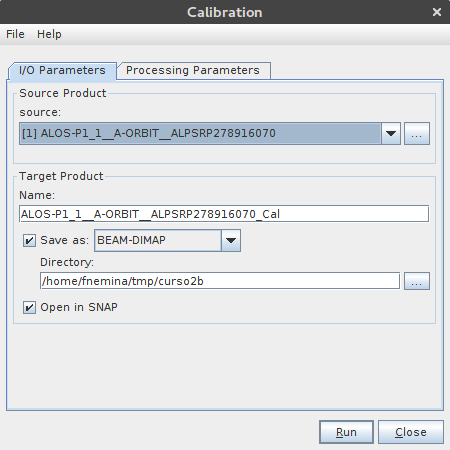
\includegraphics[width=0.35\textwidth]{fig:calibrar1.png}}
    \hspace{1cm}
    \subfloat[Processing parameters]{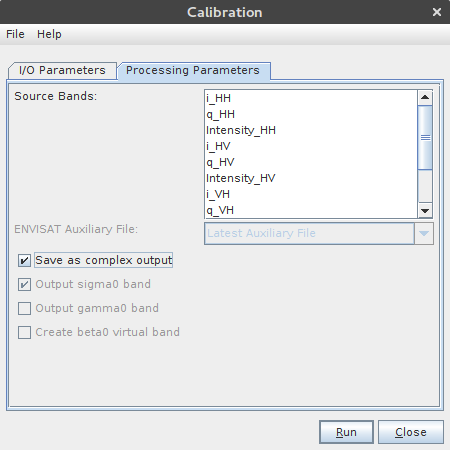
\includegraphics[width=0.35\textwidth]{fig:calibrar3.png}}
    \caption{Calibración de productos SAR utilizando el SNAP. Recuerde seleccionar en este caso la opcíon \emph{Save as complex output}.}
    \label{fig:calibrar-2}
\end{figure}

\subsection{Cálculo de matriz de coherencia}

Para calcular la matriz de coherencia, una vez calibrada la imagen, utilice la herramienta \menu{Radar>Polarimetric>Polarimetric matrix generation}.

Seleccione la imagen \directory{ALOS-P1\_1\_\_A-ORBIT\_\_ALPSRP278916070\_Cal} y en Processing parameters elija en \emph{Polarimetric Matrix} la opción \texttt{T3}. Por el momento, no se preocupe por el significado de esta matriz (Figura \ref{fig:t3}).

\begin{figure}[h!]
    \centering
    \subfloat[I/O Parameters]{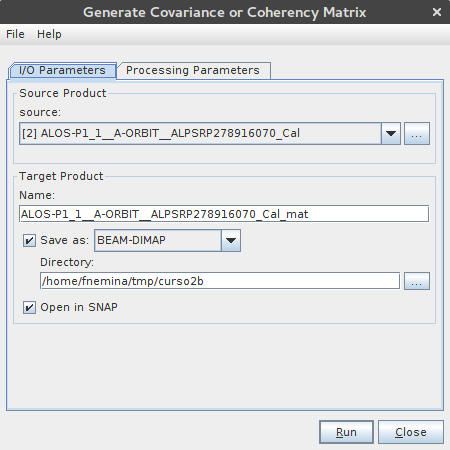
\includegraphics[width=0.35\textwidth]{fig:t31.png}}
    \hspace{1cm}
    \subfloat[Processing parameters]{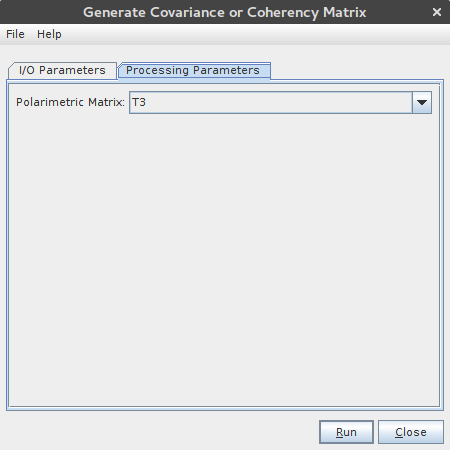
\includegraphics[width=0.35\textwidth]{fig:t32.png}}
    \caption{Cálculo de matrices polarimétricas en el SNAP.}
    \label{fig:t3}
\end{figure}

\subsection{Filtrado}

En el caso de imágenes full polarimetricas se pueden aplicar distintos tipos de filtros. Diríjase a \menu{Radar>Polarimetric>Polarimetric speckle filter}. Utilice en este caso el filtro \menu{Refined Lee Filter} en \emph{Speckle filter} sobre la imagen (Figura \ref{fig:plee})
\begin{center} \texttt{ALOS-P1\_1\_\_A-ORBIT\_\_ALPSRP278916070\_Cal\_mat}\end{center}

\begin{figure}[h!]
    \centering
    \subfloat[I/O Parameters]{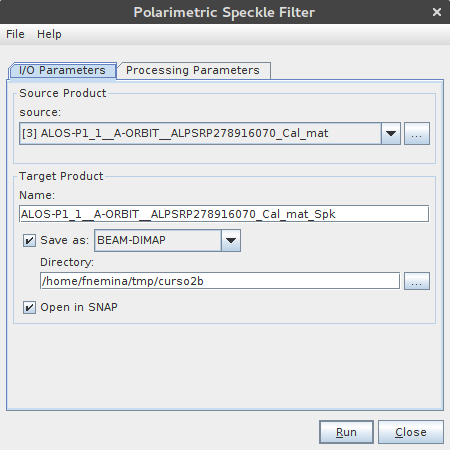
\includegraphics[width=0.35\textwidth]{fig:plee1.png}}
    \hspace{1cm}
    \subfloat[Processing parameters]{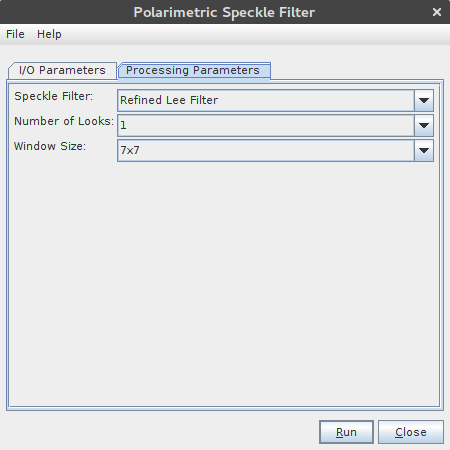
\includegraphics[width=0.35\textwidth]{fig:plee2.png}}
    \caption{Filtro \emph{Refined Lee Filter} para imágenes full polarimétricas.}
    \label{fig:plee}
\end{figure}

\subsection{Proyección}

Reproyecte la imagen en el terreno (GTC) aplicando los procesos de \emph{Deskewing} y proyección sobre un modelo de elevación digital.

\section{Descomposición de Pauli}

La descomposición de Pauli permite separar la información sobre interacciones de tipo doble rebote, en volumen y especulares, en una imagen \emph{full polarimétrica}

La descomposición genera tres bandas que suelen mostrarse de la siguiente manera:

\begin{itemize}
    \item Azul: Información por procesos de un solo rebote o un número impar de rebotes.
    \item Verde: Información por procesos de scattering en volumen.
    \item Rojo: Información por procesos de doble rebote o un número par de rebotes.
\end{itemize}

Diríjase a \menu{Radar>Polarimetric>Polarimetric Decomposition}. Seleccione como entrada la imagen corregida en terreno y la descomposición \texttt{Pauli Decomposition} en \texttt{Processing parametric} (Figura \ref{fig:pauli})

\begin{figure}[h!]
    \centering
    \subfloat[I/O Parameters]{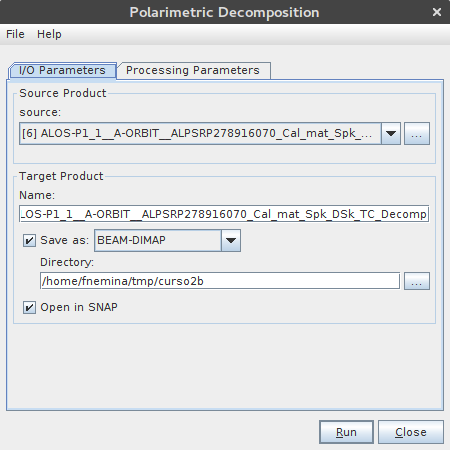
\includegraphics[width=0.35\textwidth]{fig:pauli1.png}}
    \hspace{1cm}
    \subfloat[Processing parameters]{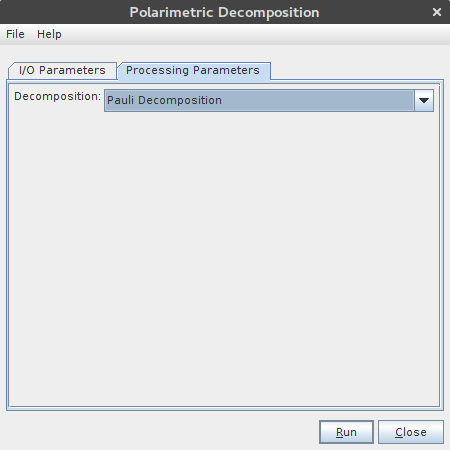
\includegraphics[width=0.35\textwidth]{fig:pauli2.png}}
    \caption{Cálculo de la descomposición de Pauli utilizando las matrices polarimétricas en el SNAP.}
    \label{fig:pauli}
\end{figure}

Observe los resultados haciendo click derecho sobre la imagen obtenida en la opción \emph{Open RGB image window} (Figura \ref{fig:pauli}).

\begin{figure}[h!]
    \centering
    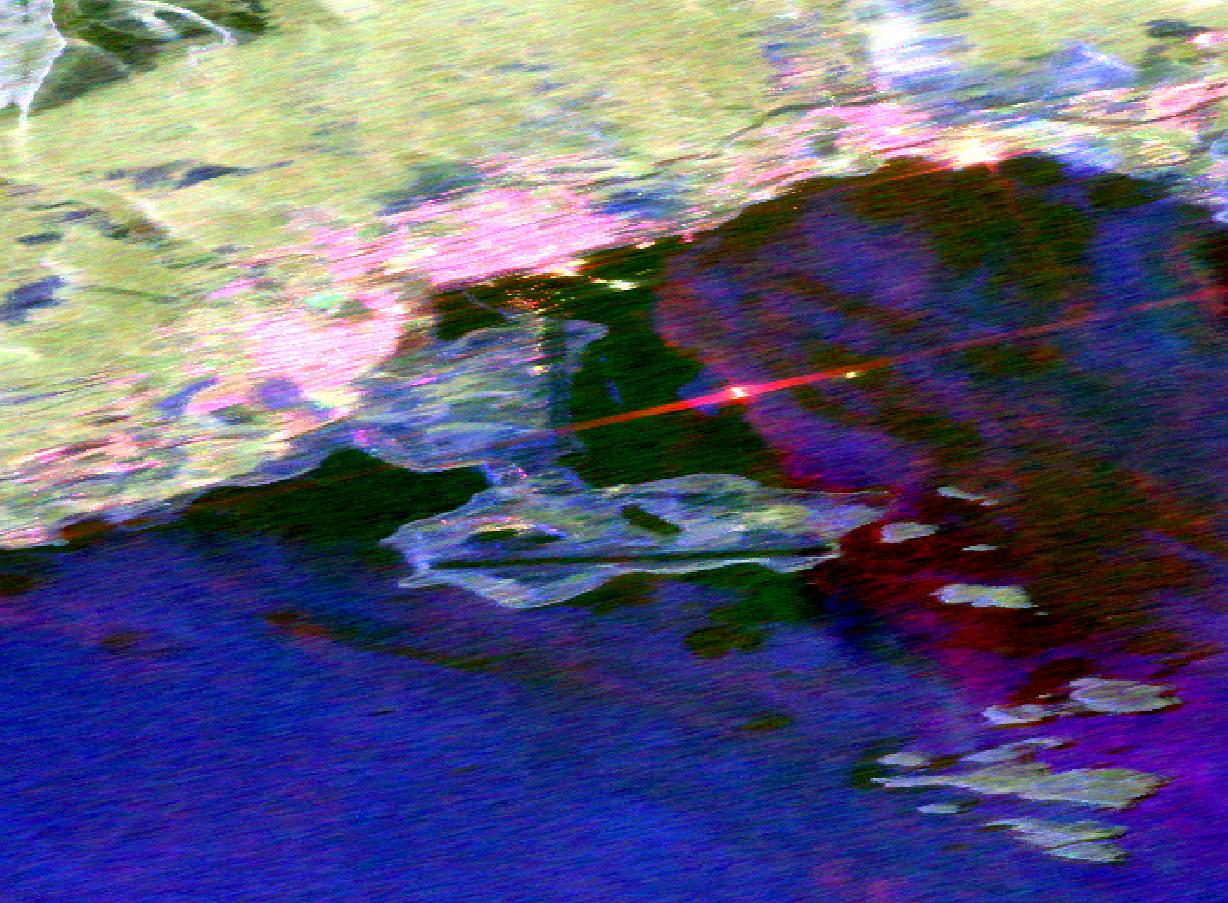
\includegraphics[width=0.7\textwidth]{fig:pauli.jpg}
    \caption{Descomposición de Pauli para la zona de interés.}
    \label{fig:pauli}
\end{figure}


\section{Preguntas para debate}

\begin{que}
    En la descomposición de Pauli, de qué color  se observan:
    \begin{enumerate}
        \item La pista de aterrizaje de la ciudad de Ushuaia.
        \item Zonas urbanas en la ciudad de Ushuaia.
        \item Zonas con vegetación sobre la ladera de la montaña.
        \item La bahía encerrada con coordenadas $54^\circ 48^\prime 51^{\prime\prime}$ latitud sur y $68^\circ 18^\prime 58^{\prime\prime}$ longitud oeste.
        \item El canal de Beagle.
    \end{enumerate}
\end{que}

Estas preguntas no serán evaluadas. Su objetivo es discutirlas en el foro de sonsultas e intercambio de la clase.
